%% This is an example first chapter.  You should put chapter/appendix that you
%% write into a separate file, and add a line \include{yourfilename} to
%% main.tex, where `yourfilename.tex' is the name of the chapter/appendix file.
%% You can process specific files by typing their names in at the 
%% \files=
%% prompt when you run the file main.tex through LaTeX.

%\providecommand{\phasezero}{Phase-0\xspace}
%\providecommand{\phaseone}{Phase-I\xspace}
%\providecommand{\phasetwo}{Phase-II\xspace}

\providecommand{\phasezero}{Phase-0}
\providecommand{\phaseone}{Phase-I}
\providecommand{\phasetwo}{Phase-II}

\chapter{Higgs pair-production}

The detailed studies of the properties of the observed Higgs
boson~\cite{AtlasPaperCombination, CMSPaperCombination,
  CMSPaperCombination2} by the ATLAS and CMS Collaborations are central components of the CERN LHC physics program. In the standard model (SM) all properties of the Higgs boson are predicted for a given mass of the Higgs boson. The present measurements of the Higgs bosons couplings to fermions and bosons and of the tensor structure of the Higgs boson interaction with electroweak gauge bosons show no
significant deviations~\cite{Khachatryan:2014jba,PhysRevD.92.012004} with respect to the SM expectations. Physics beyond the SM (BSM) can potentially lead to deviations from the SM predictions. 

Studies of Higgs boson pair production at the High-Luminosity LHC (HL-LHC) will provide
insight on the  Higgs boson trilinear coupling~\cite{Glover:1987nx,Plehn:1996wb,Djouadi:1999rca,Gianotti:2002xx,Baur:2003gpa,Baur:2003gp,Baglio:2012np}. 
This measurement would directly probe the Higgs field potential since the self-coupling is related to the third derivative of the Higgs potential at its minimum. The process is also
sensitive to other BSM effects, as new physics can modify the rate of the production. The dominant Higgs boson pair production mode at the LHC is through gluon fusion. Figure~\ref{fig:feynman} shows the 
dominant Feynman diagrams. Di-Higgs boson events can be produced via a box
diagram and through the Higgs boson self-coupling contribution. The two
processes interfere destructively and the cross section is near
minimum for the SM. The Higgs boson pair production cross  section
is about $1000$ times smaller than the single Higgs boson production cross
section. It should be noted that the cross section increases
by a factor of two if the Higgs boson self coupling is zero.  

\begin{figure}[hbtp]
  \begin{center}
    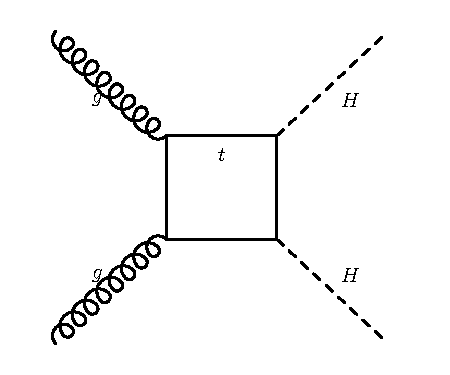
\includegraphics[width=0.49\textwidth]{figures_chapter6/hhbox.pdf}
    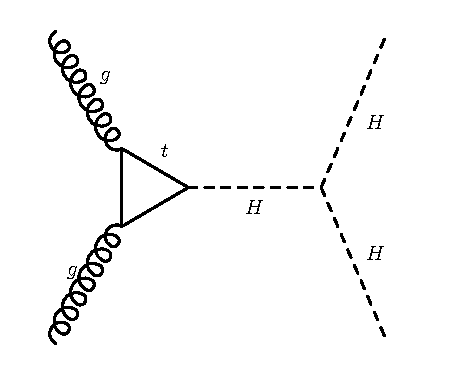
\includegraphics[width=0.49\textwidth]{figures_chapter6/hhself.pdf}       
    \caption{Feynman diagrams contributing to gluon fusion Higgs boson pair production.}
    \label{fig:feynman}
  \end{center}
\end{figure}

The gluon fusion production cross section for the Higgs boson pair production at a center of mass energy of $14$~TeV has been calculated to next-to-next-to-leading-order to be $40.7$~fb~\cite{Dawson:1998py,Grigo:2014jma}. Other production modes potentially add another $10\%$ to the total production cross section, but have not been included in this study. A large amount of integrated luminosity is required in order for these processes to be observed and measured. The signal events that are expected to be produced per experiment at HL-LHC with $3000$~$\mathrm{fb}^{-1}$ integrated luminosity are approximately $320$, $9000$, and $1500$ events for $bb\gamma\gamma$ and $bb\tau\tau$ respectively.

The increased instantaneous luminosity required to reach this target is expected to be accompanied by a significant increase in the number of overlapping inelastic collisions (pileup). The HL-LHC is expected to operate with an average of $140$ simultaneous pileup events. This presents a serious challenge to the experiments in their ability to deal with this increased level of activity and energy flow, and to preserve the detector performance under this environment. 

As part of a comprehensive strategy to address these issues, CMS has released a technical proposal for the \phasetwo upgrade~\cite{Butler:2020886} program. The expected performance of this detector at HL-LHC is assumed for these studies and is discussed in the following sections. The impact of some of the individual components of the \phasetwo upgrade on the results are highlighted where it is appropriate. In addition, the $bb\gamma\gamma$ results are also shown assuming the detector performance of the so called \phaseone CMS upgrade~\cite{Collaboration:1355706} detector after an assumed integrated luminosity of $1000$~$\mathrm{fb}^{-1}$, configuration hereafter denoted as ``\phaseone aged''.

At present, the \phasetwo detector simulation includes the upgraded outer tracker, muon systems, and calorimetry. The pixel detector upgrade, however, is still not finalized so the simulation contains the \phaseone pixel detector in the barrel and an extended version of the current pixel detector in the forward detector to provide tracking at higher $\eta$. The primary and secondary vertex reconstruction and identification performance will certainly be better
than what is assumed in these studies and should be viewed as a conservative estimate.

\section{Experimental setup and simulation}
\label{sec:exp_cond}
It is crucial that the \phasetwo detector can cope with the challenging environment of HL-LHC, as pileup mitigation, b-tagging, tau-tagging, photon identification efficiencies, and mass 
resolutions are fundamental to perform measurements on Higgs boson pair production. Triggers are assumed to be $100\%$ efficient in these studies. The \textsc{Delphes} fast simulation framework~\cite{deFavereau:2013fsa} is used 
for $bbWW$ results to model the \phasetwo detector. The parameterized performance of the \phasetwo detector in Delphes is taken from the corresponding GEANT-based~\cite{Agostinelli:2002hh} full simulation  samples. The $bb\gamma\gamma$ analysis uses Monte Carlo (MC) generator information with smearing functions to model the performance of the detector. A combination of the two approaches mentioned above is used for the $bb\tau\tau$ final state.  

Only the dominant gluon fusion inclusive production mode is produced in the signal generation. The samples are generated with \textsc{madgraph5.2}~\cite{Alwall:2011uj}, at leading order (LO), using the results from~\cite{Frederix2014142}, interfaced with  \textsc{pythia6.4}~\cite{PYTHIA} for parton showering and fragmentation. The generator is also interfaced with TAUOLA~\cite{tauola} for the simulation of the tau lepton decays. The pileup events are simulated in the Delphes samples by randomly placing minimum-bias interactions along the beam axis according to a longitudinal spread taken from the full simulation samples.


\section{$bb\gamma\gamma$ final state}

\subsection{Object selection and performance}
\label{sec:objects}

% For the remaining backgrounds we generate samples using MADGRAP 5~\cite{Alwall:2011uj}, perform the parton showering and
%hadronization using Pythia~\cite{PYTHIA}, and then apply weights to account for the object selection efficiencies
%and fake rates.
 %The efficiency for electrons to be mis-identified as photons is estimated from full simulation
%of the current Run1 CMS detector and is found to be about $1\%$ in the barrel, and $3\%$ in the endcap.
% 
The signal events of interest contain two high transverse momentum ($p_{T}$) photons and two high $p_{T}$ jets originating from b quarks. The photons are rejected if an electron is reconstructed within a distance $\Delta R = \sqrt{\smash[b]{(\Delta\eta)^2 + (\Delta\phi)^2}}$ (where the $\phi$ is azimuthal angle in radians and $\eta$ is the pseudorapidity) of $0.1$ to the photon.  A $p_{T}$ and $\eta$ dependent efficiency is applied to the photons to model the identification and isolation efficiency. The efficiency is about $80\%$ in the barrel, and about $55\%$ in the endcap. The lower efficiency in the endcap is primarily due to the electron veto requirement. The processes involving jets faking photons are among the dominant backgrounds. The rate to misidentify photons, typically referred to as the fake rate, is about $1 \times 10^{-4}$ for gluon jets and about $5\times 10^{-4}$ for quark jets. The rate to misidentify electrons as photons is taken to be as $1\%$ ($3\%$) in barrel (endcap). Di-photon mass width of $1.2$~GeV is achieved with the upgraded detector, for the events where both photons are in the barrel, using sophisticated multivariate techniques to calibrate the photon energy.  
Jets are reconstructed using the anti-kt clustering algorithm~\cite{antikt} with the resolution parameter equal to $0.5$,
and corrected for pileup effects using the FastJet technique~\cite{CMS-PAS-JME-10-003,CMS-DP-2013-011}. Standard CMS jet energy corrections for non-uniformities in $\eta$ and $p_{T}$ are applied. Jets are tagged as originating from a b quark  on the basis of the presence of secondary vertices and large impact parameter tracks, which are exploited for b-tagging in a Combined Secondary Vertex discriminator (CSV)~\cite{CMS:BTagPaper,CMS-PAS-BTV-13-001,CMS-DP-2013-005}. The chosen working point of the CSV discriminator gives, on average, b-tagging efficiencies of about $75\%$ and $65\%$ in the central and forward regions, respectively; with mistagging rates for light and charm
jets of about $1\%$ and $20\%$, respectively. Di-jet mass resolution of about $20$~GeV is achieved with the upgraded detector. 

Electrons and muons with $p_{T}>10$~GeV are selected for the purpose of vetoing events with signatures consistent with a Higgs boson produced in association with a top and anti top quark pair ($t\bar{t}H$). This process contributes
significantly to the total background after signal event selection requirements. A non-negligible fraction of such background events contain leptons and can be rejected on this basis. Very loose selection requirements with efficiency in the range between $90\%$ and $95\%$ are placed on the electron and muon candidates in order to suppress this background as much as possible.

%Photons are selected using a robust selection approach, applying requirements on the
%electromagnetic cluster width, the ratio of energies deposited in the hadronic and electromagnetic calorimeters, and isolation~\cite{CMS-DP-2013-010}. 
%A set of tight selection requirements is chosen as the processes involving jets faking photons are among the dominant backgrounds. 

\subsection{Signal and background estimation}
\label{sec:bkgestimation}
The signal process of interest is the production of two Higgs bosons, one of which decays to a pair of b quarks, 
and the other decaying to a pair of photons. The main resonant backgrounds are $ZH$, where a Higgs boson is produced in association
with a Z boson which subsequently decays to two b-jets, $t\bar{t}H$, where a Higgs boson is produced
in association with a top and anti-top quark pair, and $b\bar{b}H$, where a Higgs boson is produced in
association with a b and anti-b quark pair. The non-resonant backgrounds include QCD production 
of $b \bar{b} \gamma\gamma$, QCD production of $jj \gamma\gamma$ with light jets mistagged 
as b-jets, QCD production of $b \bar{b} j \gamma$ and $b \bar{b} jj$ with one and two
jets mis-identified as photons respectively, and QCD production of four jets with two jets mis-identified 
as photons and two jets mistagged as b-jets, dominated by mistagged charm jets. 
These background processes have cross sections that are several orders of magnitude larger than the resonant backgrounds, but are suppressed
by the low rate for mistags and mis-identified photons. Due to their large cross sections,  it is computationally impossible to fully simulate these background events. Instead, we adopt the approach of producing generator particle level Monte Carlo (MC) samples and weighting the events by the corresponding efficiencies and fake rates for selecting the constituent particles. Finally, SM  production of $t\bar{t}(\gamma)$ enters as background for our signal event selection
for events where both top quarks decay semi-leptonically to electrons and one (or both) of the electrons are mis-identified as photons. A sample of di-electron decays of the $t\bar{t}(\gamma)$ events are weighted by the corresponding electron to photon mis-identification rates to estimate the background contribution.

The cross sections for non-resonant background processes are summarized in Table~\ref{tab:CrossSections}. Recent studies of the non-resonant background production of $b \bar{b} \gamma\gamma$ show that the rate is significantly enhanced when full next-to-leading order (NLO) simulation is performed~\cite{Azatov:2015oxa}. The NLO simulation includes both the real and virtual corrections. The k-factor is about $2$ and this is included in the table.  


\begin{table}[!ht]
\begin{center} 
\begin{tabular}{|c|c|}
\hline
Process                                           &   Cross Section (fb)   \\ \hline
$b \bar{b} \gamma\gamma$                          &   $272$                            \\
$jj \gamma\gamma$                                 &   $2.2 \times 10^{4}$              \\
$bb j\gamma$                                      &   $8.1 \times 10^{5}$              \\
$cc j\gamma$                                      &   $2.5 \times 10^{6}$              \\
$bb jj$                                           &   $6.1 \times 10^{8}$              \\
$cc jj$                                           &   $6.5 \times 10^{8}$              \\
$jjjj$                                            &   $2.0 \times 10^{10}$             \\ \hline
\end{tabular}
\caption{ The production cross section of the non-resonant background processes at a center of mass energy 
of $14$~TeV are shown.}
\label{tab:CrossSections}
\end{center}
\end{table}

\subsection{Event selection}
\label{sec:eventselection}
 
Events containing two photons with $p_{T}$ greater than $25$~GeV
and $|\eta|<2.5$, and two b-agged jets with $p_{T}$ greater than $30$~GeV and $|\eta|<2.4$ are selected. While the \phasetwo upgrades allow b-jet tagging capabilities up to $|\eta|$ ranges of $3.0$, the b-tagged jets with $p_{T}$ greater than $30$~GeV for the signal events are predominantly central and therefore only $|\eta|<2.4$ is required. One of the two photons is required to have $p_{T} > 40$~GeV. Due to the large amount of background from jets faking photons in the endcap region of the detector the event sample is split up into two categories, one with both photons and in the barrel and one
with at least one photon in the endcap. To suppress $t\bar{t}H$ background
events, it is required that there are no electrons or muons passing the veto selection and that 
the number of jets with $p_{T}>30$~GeV and $|\eta|<2.5$ is less than four. 

A number of different additional kinematic requirements were investigated in order to improve the signal to background ratio. It is required that the $\Delta R$ between the two photons and the $\Delta$R between the two b-jets are less than $2.0$, and that the minimum of the 
$\Delta R$ between photons and b-jets is larger than $1.5$. With the above kinematic selection requirements, a signal to background ratio of about $1:3$ is achieved.

The expected event yields for the signal and resonant background processes, and the 
non-resonant background processes for various stages of the event selection
are shown in Table~\ref{tab:EventYields}. For the event category with both photons
in the barrel, the dominant backgrounds are $bb\gamma\gamma$, $jj\gamma\gamma$ primarily
consisting of mis-tagged charm jets, and $bbj\gamma$ with one fake photon, while for the
event category with at least one photon in the endcap the dominant backgrounds are
$bbj\gamma$ and $bbjj$ with one or two fake photons.


\begin{table}[!ht]
\begin{center} 
\begin{tabular}{|c|c|c|c|c|}
\hline
Process / Selection Stage            &  $HH \rightarrow b\bar{b}\gamma\gamma$  &  $ZH \rightarrow b\bar{b}\gamma\gamma$ &  $t\bar{t}H \rightarrow W W b \bar{b}\gamma\gamma$ &  $b\bar{b}H$                   \\  \hline
Object Selection \&                  &  \multirow{2}{*}{23.8 (6.27)}            &  \multirow{2}{*}{30.5 (12.0)}           &  \multirow{2}{*}{184 (47.2)}                      &  \multirow{2}{*}{6.53 (2.61)}    \\ 
Fit Mass Window                      &                                         &                                        &                                                    &                                \\ 

Kinematic Selection                  &  13.4 (3.27)                             &  15.1  (4.44)                            &  3.39  (1.04)                                        &  2.09 (0.78)       \\ 
Mass Windows                         &  9.00 (1.91)                              &  3.39  (0.26)                            &  1.57 (0.26)                                         &  0.78 (0.26)       \\  \hline

\end{tabular}

\vspace{2mm}

\begin{tabular}{|c|c|c|}
\hline
Process / Selection Stage           &  $b \bar{b} \gamma\gamma$   & $jj \gamma\gamma$            \\  \hline
Object Selection \&                 &  \multirow{2}{*}{2767 (1363)} & \multirow{2}{*}{954 (552)} \\ 
Fit Mass Window                     &                             &                              \\ 
Kinematic Selection                 &  162  (88.8)                 &  30.2  (19.7)                      \\ 
Mass Windows                        &  10.4 (5.70)                &  2.1 (1.2)                     \\  \hline
\end{tabular}

\vspace{2mm}

\begin{tabular}{|c|c|c|c|c|c|}
\hline
Process / Selection Stage           &  $bb j\gamma$                  &  $ccj\gamma$                  & $bb jj$                    &  $ccjj$ \& $jjjj$                       & $t\bar{t}(\gamma)$                \\  \hline
Object Selection \&                 &  \multirow{2}{*}{1592 (5145)}   &  \multirow{2}{*}{27.2 (46.3)}   & \multirow{2}{*}{279 (1622)} &  \multirow{2}{*}{7.8 (44.4)}  &  \multirow{2}{*}{597 (705)} \\ 
Fit Mass Window                     &                                &                               &                            &                               &                           \\ 
Kinematic Selection                 &  96.9  (351)                     &  0.7  (3.7)                   & 19.6 (137)                   &  0.2 (2.1)                    &  21.5 (20.3)                \\ 
Mass Windows                        &  6.3 (17.2)                     &  0.0  (0.2)                   & 1.1 (7.9)                 &  0.02 (0.1)                   &  1.2 (1.2)                \\  \hline
\end{tabular}

\caption{ The expected event yields of the signal and background processes
for $3000$~$\mathrm{fb}^{-1}$ of integrated luminosity
are shown at various stages of the cut-based selection for 
the category with both photons in the barrel. The event yields for the category with at least one photon in the endcap are shown inside the brackets. A large fit mass
window, $105$~GeV to $145$~GeV for $\mathrm{M}_{\gamma\gamma}$ and $70$~GeV to $200$~GeV for $\mathrm{M}_{bb}$,
is used for the likelihood fit analysis described in Section~\ref{sec:signalextraction}. }
\label{tab:EventYields}
\end{center}
\end{table}


\subsection{Signal extraction}
\label{sec:signalextraction}

To extract the signal and cross section, the kinematic selection requirements from Section~\ref{sec:eventselection} are applied, and  a two dimensional maximum
likelihood fit on the di-photon and di-bjet mass distributions is performed. Probability density functions (PDF's) are derived for the di-photon mass, $\mathrm{M}_{\gamma\gamma}$, and di-bjet mass, $\mathrm{M}_{bb}$
distributions for the signal, the resonant background, and the non-resonant background by 
fitting the distributions from the Monte Carlo simulation samples to particular parametrization 
of the line-shape for $\mathrm{M}_{\gamma\gamma}$ and $\mathrm{M}_{bb}$. The distributions of the signal and resonant backgrounds are fitted with a Crystal Ball distribution, while for
the non-resonant backgrounds are fitted to a decaying exponential. 
%The $\mathrm{M}_{bb}$ distribution 
%for the signal and resonant backgrounds, dominated by ZH where the Z boson decays into a pair of b jets,
%is fitted with a Crystal Ball distribution, and the $\mathrm{M}_{bb}$ distribution for the non-resonant background is
%fitted with a decaying exponential. 
To model the degraded jet energy resolution under the HL-LHC pileup conditions, the jet energy resolution parameter is then appropriately increased.
 
%We check for correlations between $\mathrm{M}_{\gamma\gamma}$ and $\mathrm{M}_{bb}$ by evaluating the correlation coefficients, 
%and find that they are at negligible levels for the signal and background processes. 
The correlations between $\mathrm{M}_{\gamma\gamma}$ and $\mathrm{M}_{bb}$ are assumed to be negligible. Therefore, the two dimensional PDF's are simply the product of the one dimensional PDF's. The expected number of events within the fit mass window is used to weight the PDF's for the signal, the resonant background, and the non-resonant background to build the full model for the signal region sample. 

Toy MC experiments are randomly drawn from the full model and two dimensional fits are performed, where the yields of the signal, the resonant background, and the non-resonant background are floated.  Figure~\ref{fig:twoDfullFitProjection} shows the projections for the event category with both photons in the barrel of one example toy experiment and the fitted result. 
The average fit uncertainty of the cross section measurement using the two
dimensional fit is about $67\%$. The expected significance is about $1.6$ standard deviations. 

\begin{figure}[h]
  \centering
  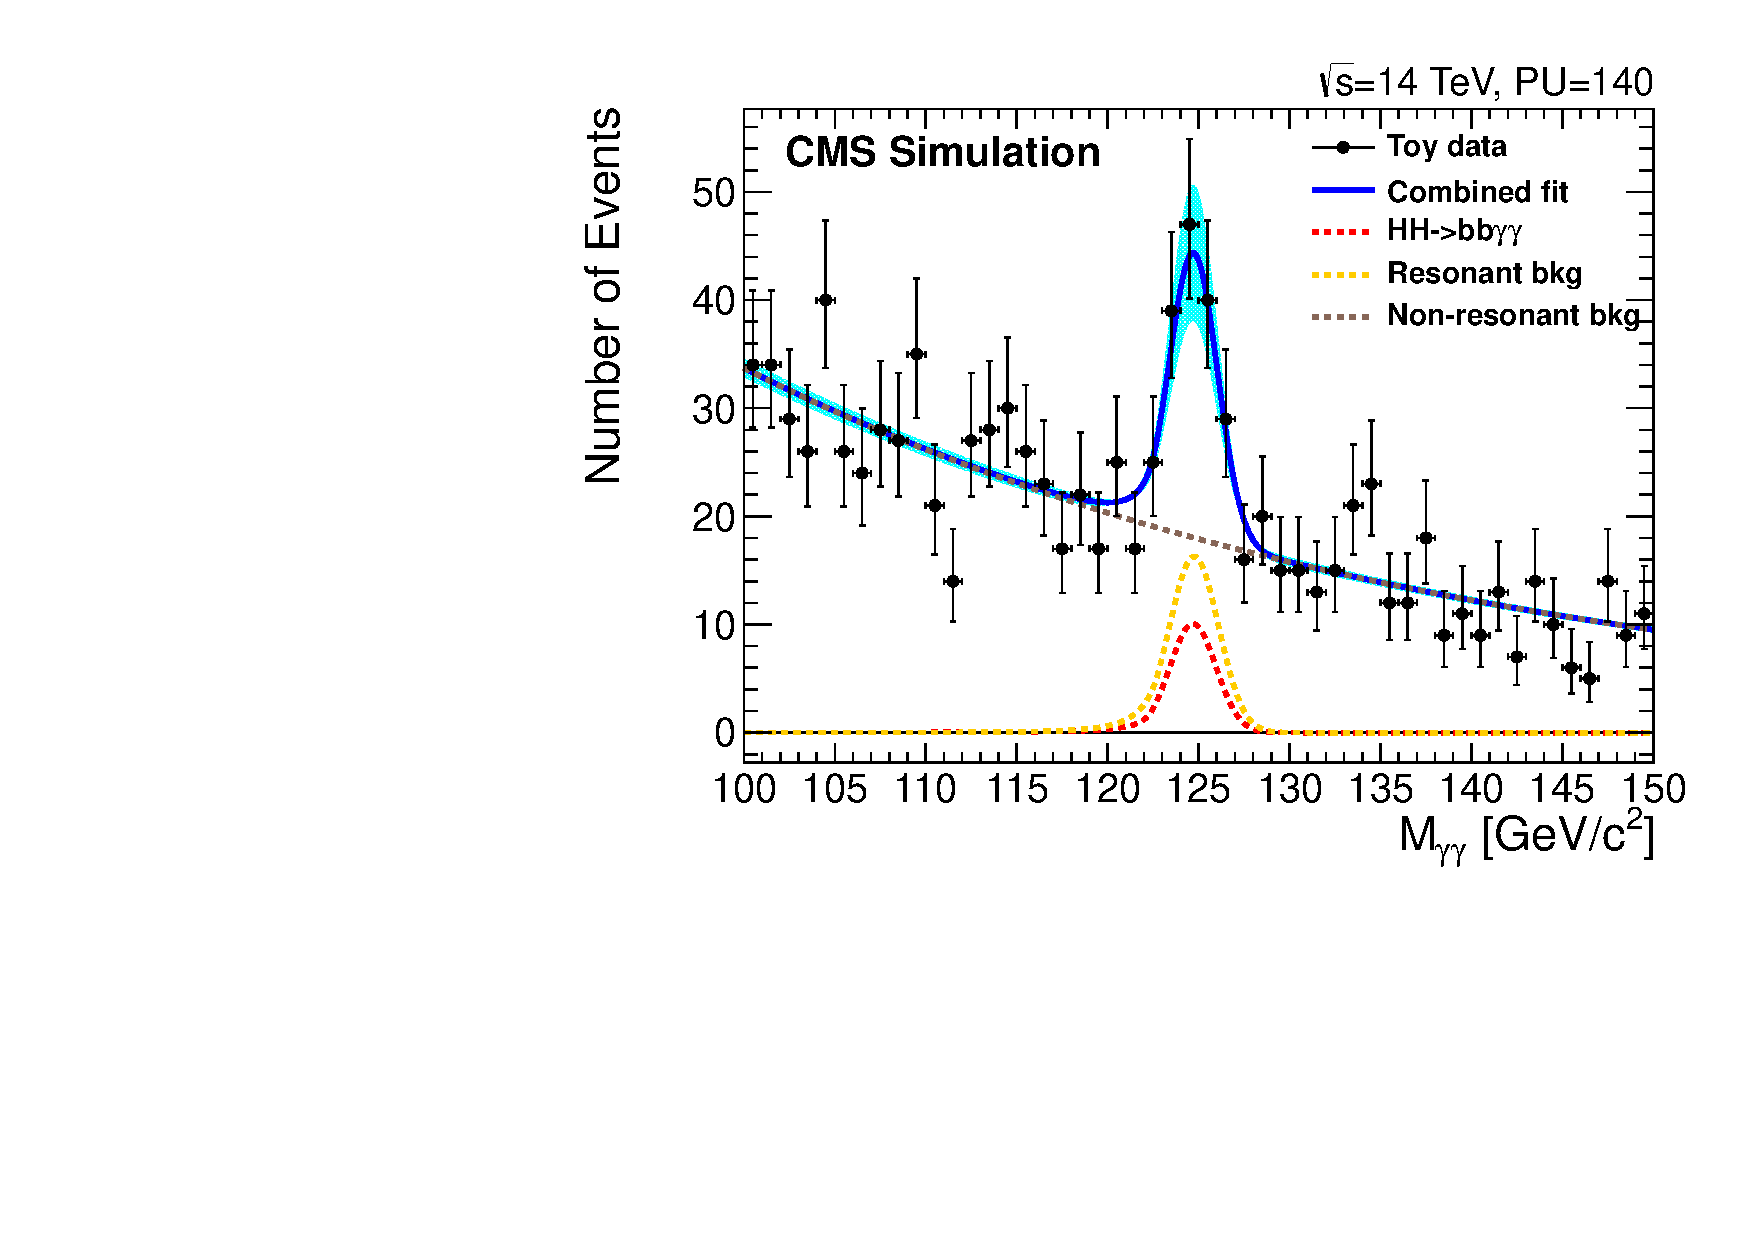
\includegraphics[width=0.9\textwidth]{figures_chapter6/hh_bbgg_mgg.pdf}
  \caption{Projections of a two dimensional fit on the di-photon mass for one representative
  toy experiment is shown. The signal, the resonant background, and the non-resonant background components are shown in 
  red, yellow, and gray, respectively.}
  \label{fig:twoDfullFitProjection}
\end{figure}


\subsection{Systematic uncertainties}

Though the statistical uncertainties dominate over the systematic uncertainties with $3000$~$\mathrm{fb}^{-1}$ of integrated luminosity, the main systematic uncertainties are discussed for completeness.
The photon selection efficiency systematic uncertainty is dominated by the systematic uncertainty in the efficiency of the electron veto requirement, and is 
less than $2\%$~\cite{CMS-DP-2013-010}. The systematic uncertainty in the b-tagging efficiency is between $2\%$ and $3\%$ depending on the $p_{T}$ and $\eta$ of the jet~\cite{CMS:BTagPaper,CMS-PAS-BTV-13-001}. 

The jet energy resolution has been measured to better than $10\%$~\cite{Chatrchyan:2011ds}, and the photon energy resolution is known to within approximately $15\%$~\cite{Chatrchyan:2013dga}. These uncertainties are propagated to the signal and background models for $\mathrm{M}_{bb}$ and $\mathrm{M}_{\gamma\gamma}$ by performing toy experiments. It is found that the average bias induced on the cross section measurement are about $2\%$ and $4\%$ for the jet energy resolution and photon energy resolution, respectively. 

The systematic uncertainty in the non-resonant background is evaluated by 
performing toy MC experiments where the assumed non-resonant background
model used is the product of an exponential and a fourth-degree polynomial fitted to
the expected non-resonant background distribution, while
an exponential function is used to perform the fit. This results in an
average bias of about $12\%$.

Finally, the systematic uncertainties in the coupling measurement arises from the 
theoretical uncertainties on the double Higgs boson production cross section. Combining
the uncertainties from missing higher order corrections, uncertainties on $\alpha_{S}$ and the PDF's, we obtain a potential change in the cross section of about $11\%$ for a center of mass energy of $14$~TeV~\cite{Baglio:2012np}.

\subsection{Upgrade scenarios}
\label{sec:scenarios}

As discussed in Section~\ref{sec:objects}, it is critical to achieve a robust reconstruction of the detector objects under the HL-LHC pileup conditions. As the measurement is primarily limited by the number of selected signal events, improving the object selection efficiency is the most important aspect. To explore the effect of the object selection efficiencies and to provide a general goal for the detector upgrade, Figure~\ref{fig:PhotonEffImprovementScan} shows the sensitivity as a function of the relative improvement on the photon selection efficiency and
the b-tagging efficiency, respectively, over the current performance estimate under the HL-LHC pileup conditions. It is seen that the measurement can be significantly improved with even a modest improvement in photon selection efficiency or b-tagging efficiency. 

\begin{figure}[h]
  \centering
  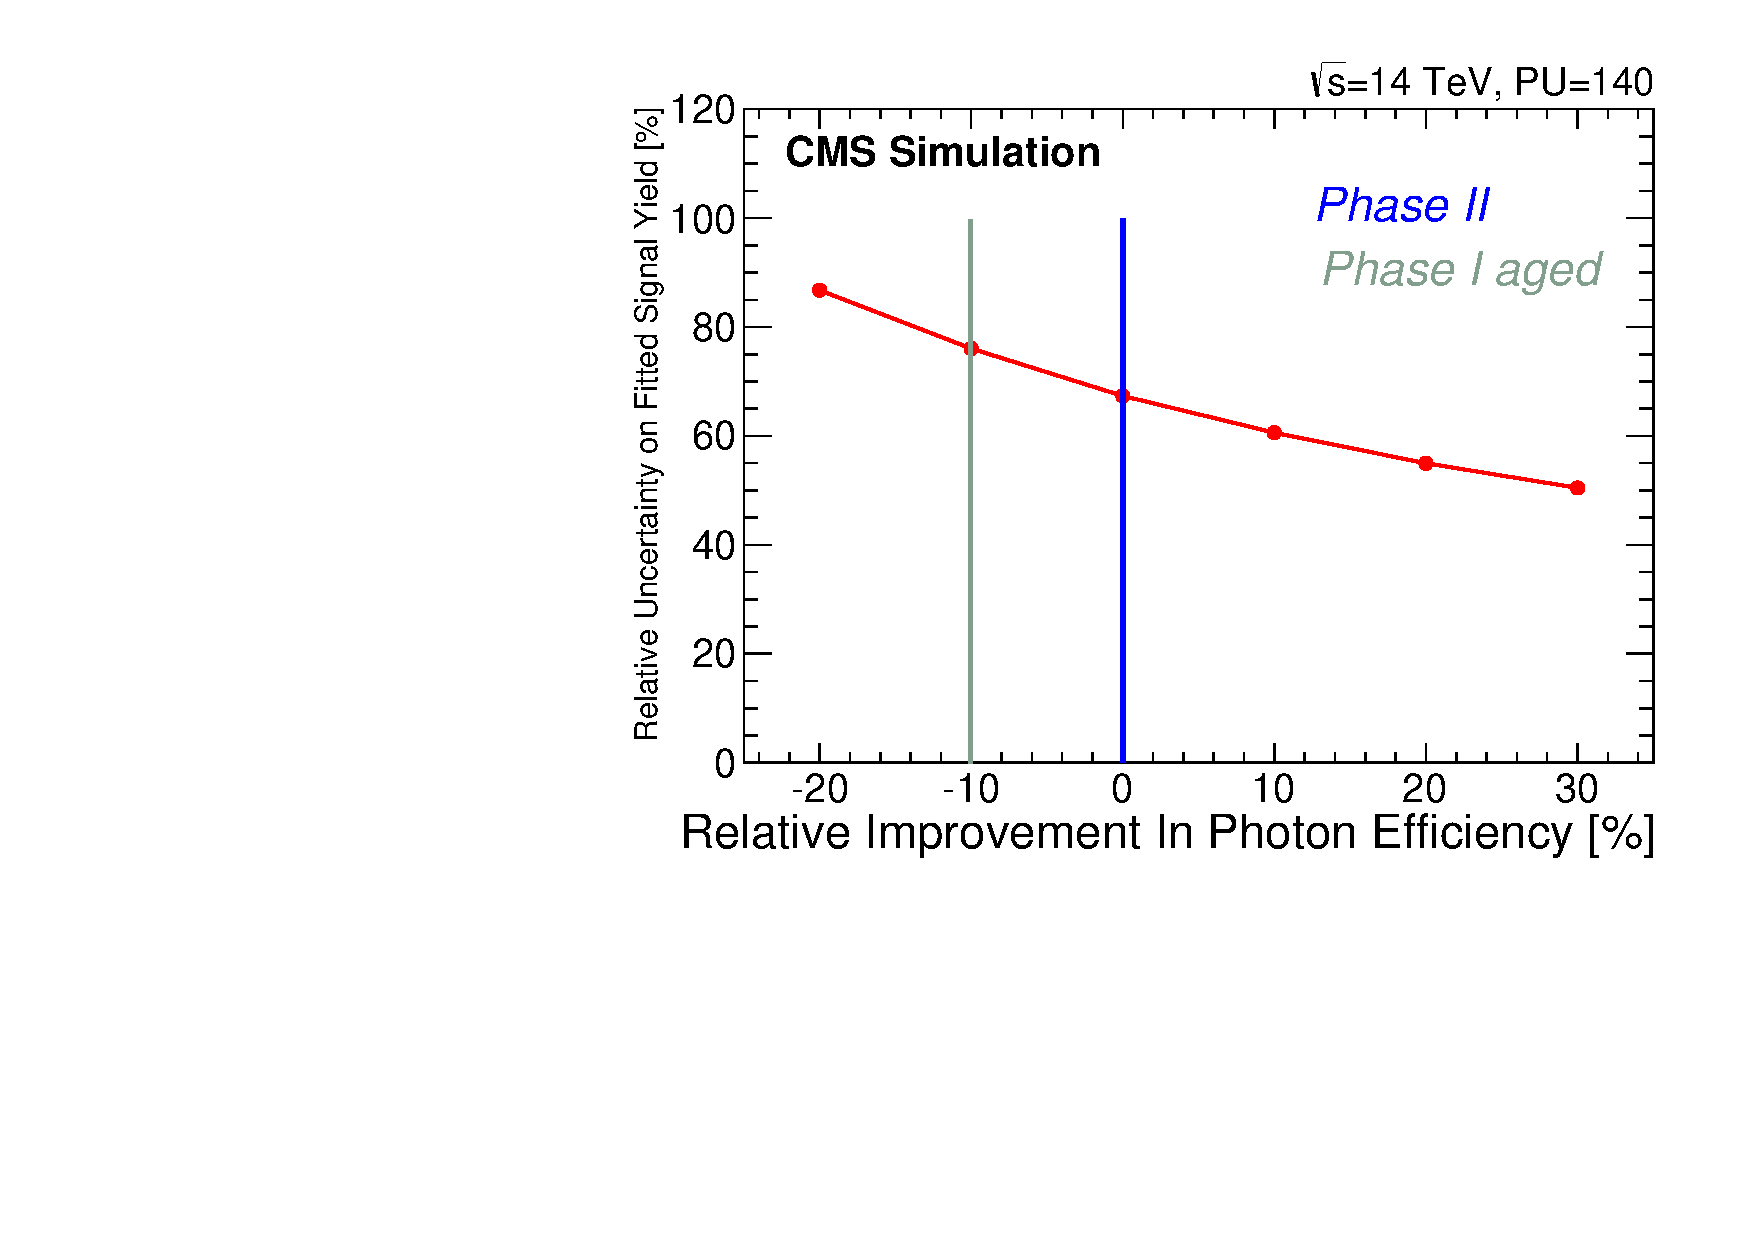
\includegraphics[width=0.49\textwidth]{figures_chapter6/XSUncertaintyVsPhotonEffRatio.pdf}
  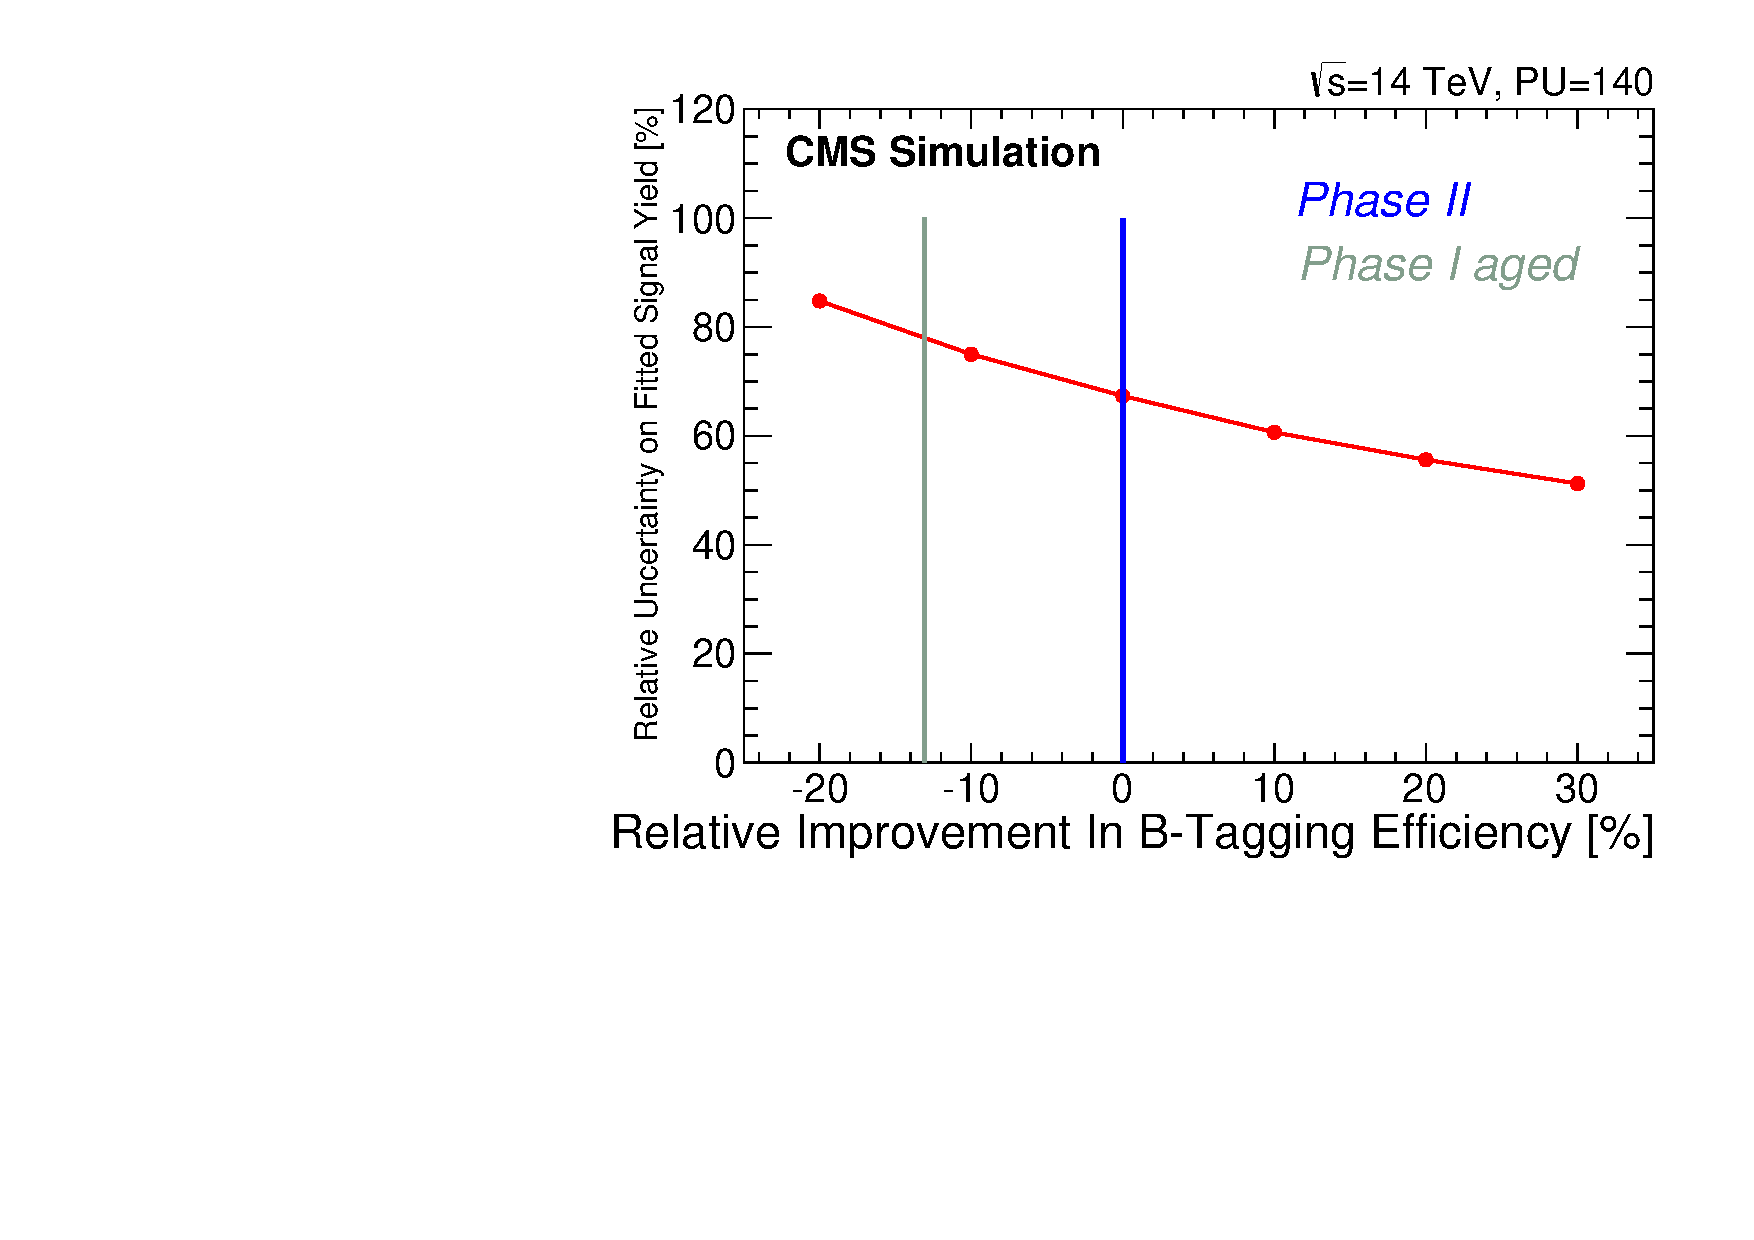
\includegraphics[width=0.49\textwidth]{figures_chapter6/XSUncertaintyVsBtagEffRatio.pdf}
  \caption{ The average expected relative uncertainty in the di-Higgs cross section measurement
  is shown as a function of the relative improvement in the photon (left) and b-tagging (right) selection efficiency 
  over the current performance estimate under the HL-LHC
  pileup conditions.}
  \label{fig:PhotonEffImprovementScan}
\end{figure}


Finally, the analysis sensitivity as a function of the total
integrated luminosity (left) and the relative contribution of the non-resonant background (right) is shown in Figure~\ref{fig:LumiScan}.

\begin{figure}[h]
  \centering
  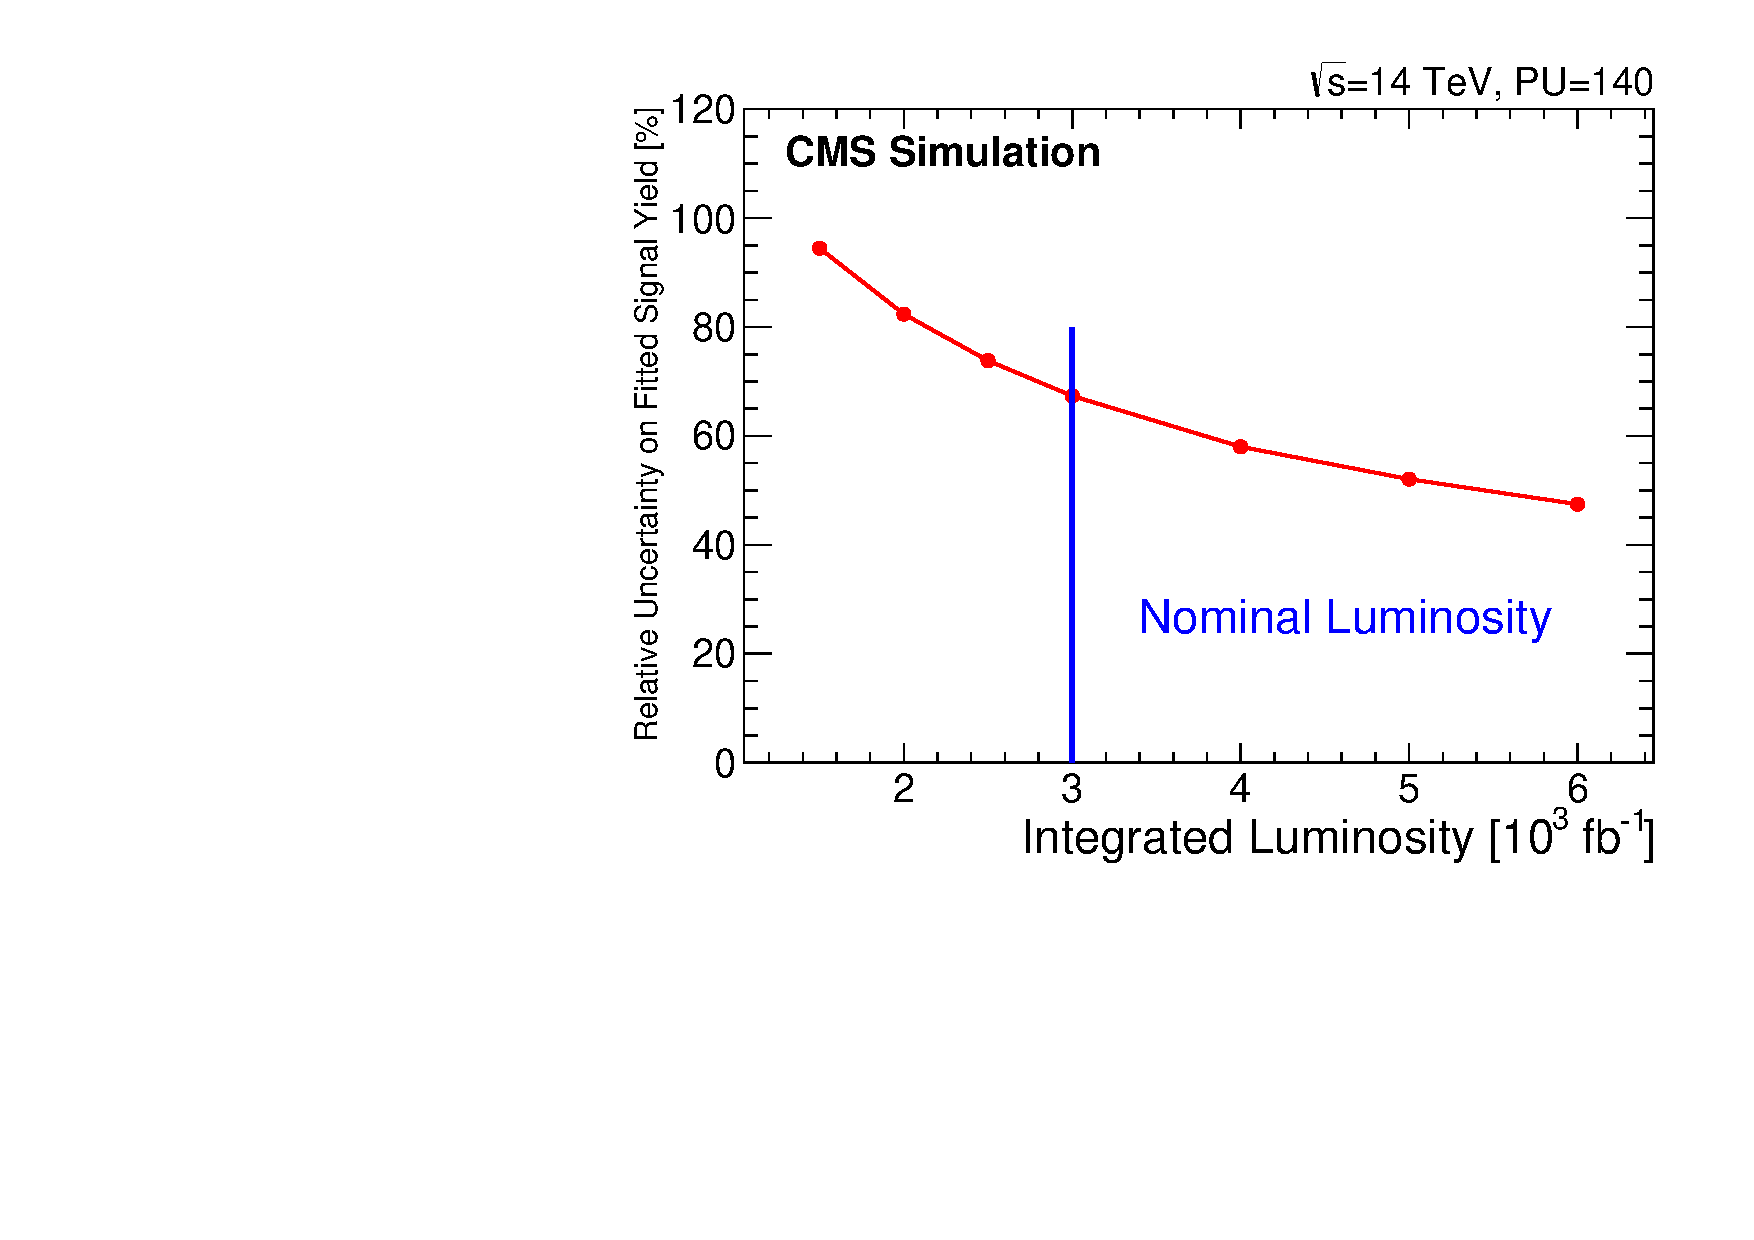
\includegraphics[width=0.48\textwidth]{figures_chapter6/XSUncertaintyVsLumi.pdf}
 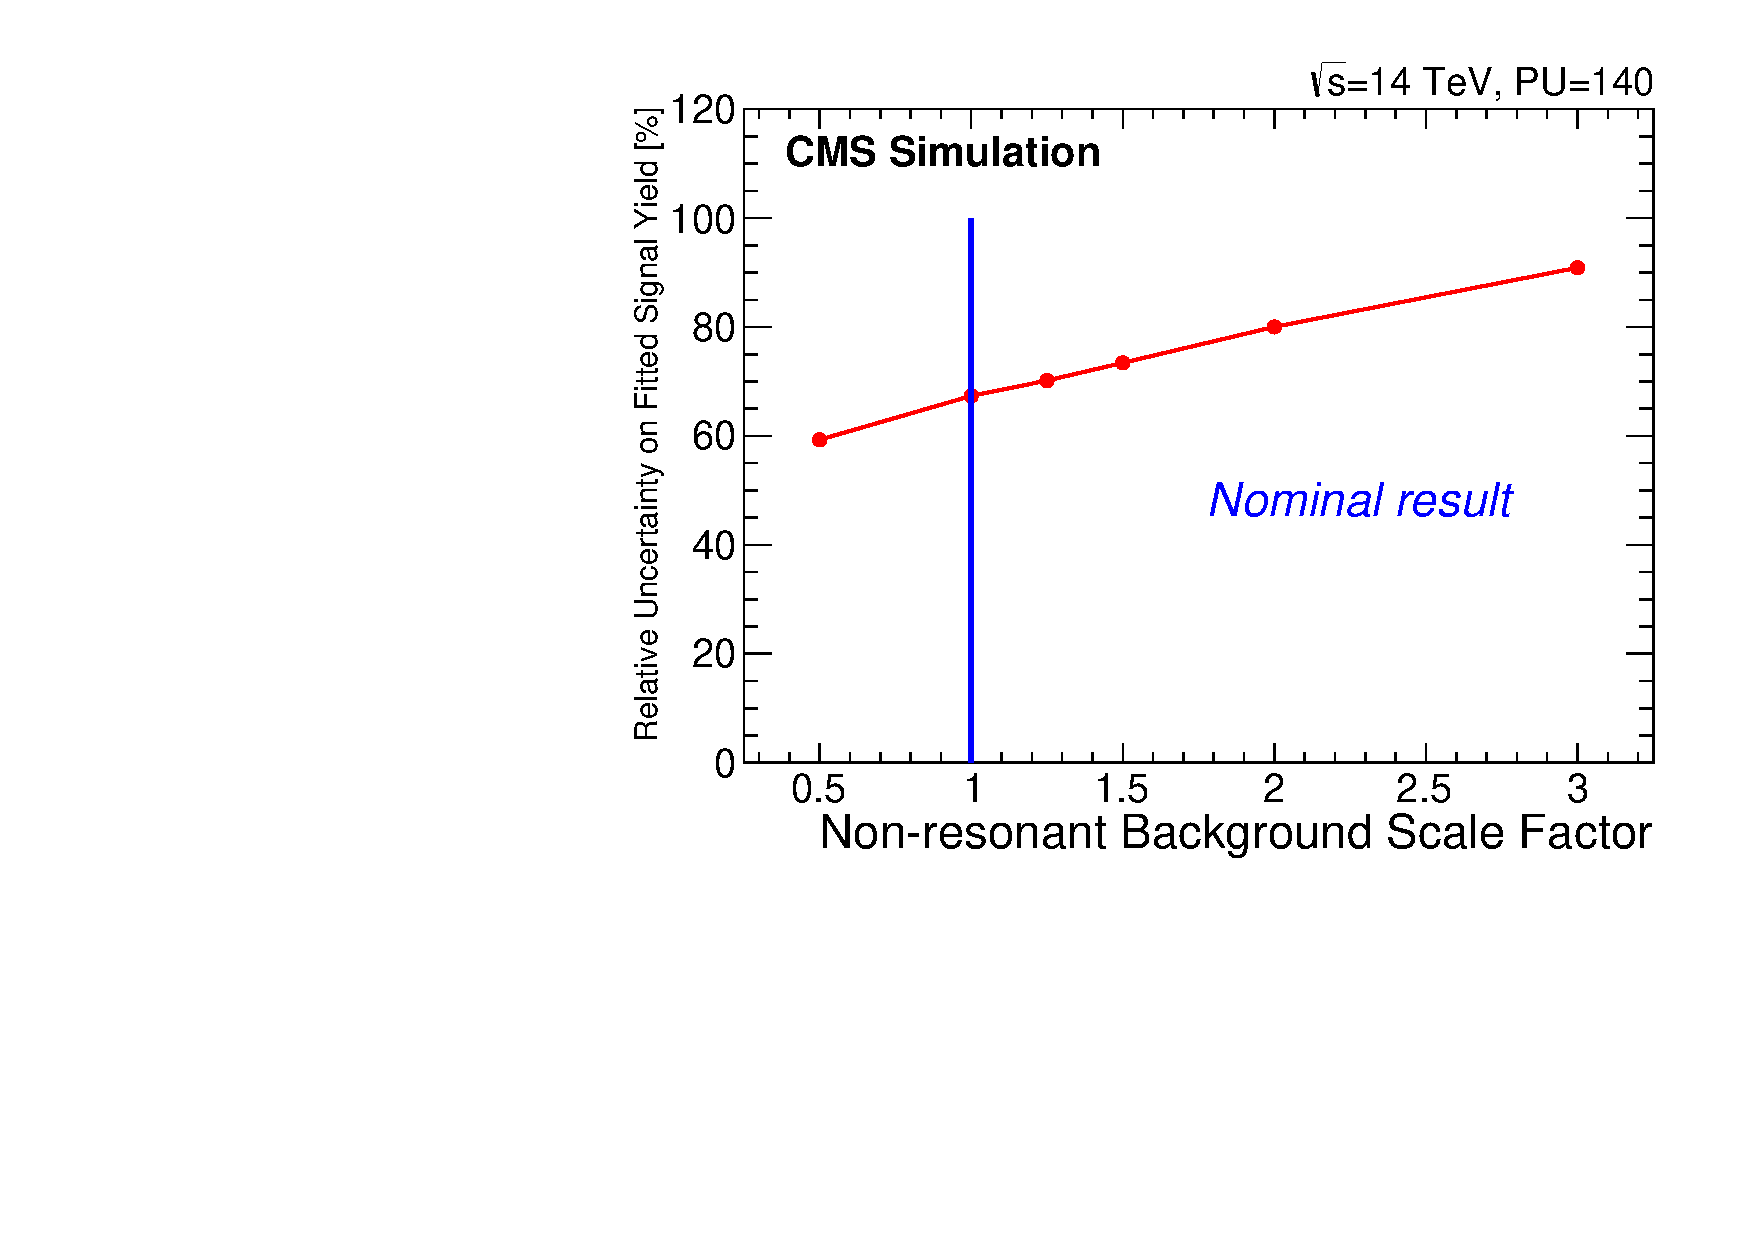
\includegraphics[width=0.48\textwidth]{figures_chapter6/XSUncertaintyVsNonResBkgScaleFactor.pdf} 
  \caption {The average expected relative uncertainty in the di-Higgs cross section measurement 
  is shown  as a function of the integrated luminosity (left) and the relative contribution of the non-resonant background.}
  \label{fig:LumiScan}
\end{figure}


\section{$bb\tau\tau$ final state}

\subsection{Object selection and performance}
The signal events of interest contain two high $p_{T}$ taus and two high $p_{T}$ jets originating from b quarks. Di-tau final states $\tau_{\mu}\tau_{h}$, and $\tau_{h}\tau_{h}$, where $h$ denotes hadronic tau decays, and $\mu$ denotes tau decays to muons, are considered.
The jets are reconstructed using the anti-kt algorithm with the resolution parameter equal to $0.4$. A cut based jet pileup identification is developed in Delphes using the track related and jet shape variables described in section 3.5.2. The efficiency of the jet pileup identification is $0.95$ with a pileup jet rate of $0.20$. The $\vec{E}_{T}^{miss}$ resolution is critical for the di-tau mass reconstruction. Without pileup mitigation the resolution is on average $50$~GeV with $140$ pileup interactions. With pileup identification the  $\vec{E}_{T}^{miss}$ resolution in Delphes is reduced to about $25$~GeV. 
The efficiency of selecting jets originating from b quarks and tau hadronic decays are parameterized in Delphes. To further reduce background events with light jets mimicking hadronic
tau decays it is required that jets originating from hadronic tau decays contain an isolated track. With the upgraded \phasetwo detector and this selection, a tau identification efficiency of about $55\%$ is possible while keeping miss-tag rates for light-jets to be less than $0.5\%$. The working point used for b-tagging has an average efficiency of $0.68$ with $0.1$ and $0.01$ mistag rates from c-quarks and light quarks respectively.  Similarly, muon efficiencies and resolutions are parameterized in Delphes and efficiencies of about $95\%$ are assumed.

\subsection{Event selection and background estimation}
Events are selected containing two b-tagged jets with $p_{T}>30$~GeV
and $|\eta|<2.4$, and two taus with $p_{T}>60$~GeV, or $p_{T}>90$~GeV
for the leading tau and $p_{T}>45$~GeV for sub-leading tau, and
$|\eta|<2.1$ for the $\tau_{h}\tau_{h}$ di-tau final state, $p_{T}>30$~GeV
and $|\eta|<2.1$  for the $\tau_{h}$ and $p_{T}>30$~GeV and $|\eta|<2.5$
for the $\tau_{\mu}$ in $\tau_{\mu}\tau_{h}$ di-tau final states. 

The background samples are simulated using the techniques that were developed for Snowmass 2013 Energy Frontier for the future hadron colliders~\cite{Avetisyan}. The existing samples were reconstructed using Delphes. A similar approach to the $bb\gamma\gamma$ analysis is adopted by producing a generator particle level $t\bar{t}$ sample and weighting the events by their corresponding efficiencies for selecting the constituent particles. The resolution effects of the detector are also taken into account. The main background is $t\bar{t}$ production with fully leptonic decays. Another source of large background is the Drell-Yan
production of a $Z$ boson decaying into a pair of tau leptons
produced in association with jets, where light jets are mis-tagged as
b-jets. The important single Higgs boson backgrounds are $ZH$ and  $t\bar{t}H$ processes. The remaining backgrounds considered are single top and $t\bar{t}$
produced in association with a vector boson, and di-boson processes.
The QCD multi-jet background is negligible in the signal region, as verified by studying the LHC data available at $\sqrt{s} = 8$~TeV. A likelihood based mass reconstruction technique (SVFIT) is used to reconstruct the di-tau mass~\cite{Chatrchyan:2014nva}. It is a powerful tool to discriminate against background processes containing a $Z$ boson that subsequently decays to tau leptons. 

\subsection {Signal extraction}
 Selections are applied on the di-tau
mass,
$M_{\tau\tau}$, and the di-b-jet mass, $M_{bb}$, distributions to identify
Higgs boson decays to tau and b pairs, respectively. The requirement
for $m_{bb}$ is $90$~GeV$<m_{bb}<130$~GeV, and
$110$~GeV$<m_{\tau\tau}<140$~GeV for $m_{\tau\tau}$. The event selection is summarized in Table~\ref{tab:event_selection} 

\begin{table}[!ht]
\begin{center} 
\begin{tabular}{|c|c|}
\hline
Event selection                                    \\ \hline
$\geq 2$ b-tagged jets with $p_{T}>30$~GeV, $|\eta|<2.4$ \\ \hline
$\tau_{h}\tau_{h}$ final state                     \\ 
$\geq 2$ isolated $\tau_{h}$-s with $p_{T}>60$~GeV or $p_{T}>90/45$~GeV, $|\eta|<2.1$  \\ \hline
$\tau_{\mu}\tau_{h}$ final state                     \\ 
An isolated $\tau_{h}$ with $p_{T}>30$~GeV, $|\eta|<2.1$ and an isolated $\tau_{\mu}$ with  $p_{T}>30$~GeV, $|\eta|<2.5$ \\ \hline 
 $90$~GeV$<m_{bb}<130$~GeV and $110$~GeV$<m_{\tau\tau}<140$~GeV \\ \hline
\end{tabular}
\caption{ Event selection summary for bb$\tau\tau$ final state.}
\label{tab:event_selection}
\end{center}
\end{table}

A kinematic bounding variable, $m_{T2}$, is introduced to further
discriminate the dominant $t\bar{t}$ background from the di-Higgs signal~\cite{smt}. By construction, $m_{T2}$ is 
bounded above by the top quark mass for $t\bar{t}$ background events
while it is unbounded for di-Higgs boson signal events. For the
$\tau_{\mu}\tau_{h}$ di-tau final states a boosted decision tree (BDT) discriminant was trained to further exploit the boosted kinematics of di-Higgs boson
production. The input variables are the masses, transverse momenta,
and $\Delta R$ distances of the di-tau, di-b-jet, and di-Higgs
systems. The $m_{T2}$ variable is also included in the
training.

Figure~\ref{fig:bdtout} shows the predicted distributions of the $m_{T2}$ variable (left) for the $\tau_{h}\tau_{h}$ final state and BDT discriminant variable (right) for the $\tau_{h}\tau_{\mu}$ final state after the mass window requirements. Both variables provide good discrimination between signal and background. As expected the $t\bar{t}$ background is bounded above by the top quark mass taking into account the detector resolution effects. Tables~\ref{tab:hhsig} and ~\ref{tab:mhsig} show the expected event yields for $3000 \mathrm{fb}^{-1}$ integrated luminosity at various stages of the event selection for the $\tau_{h}\tau_{h}$, and $\tau_{\mu}\tau_{h}$ channels, respectively. 

\begin{figure}[hbtp]
\begin{center}
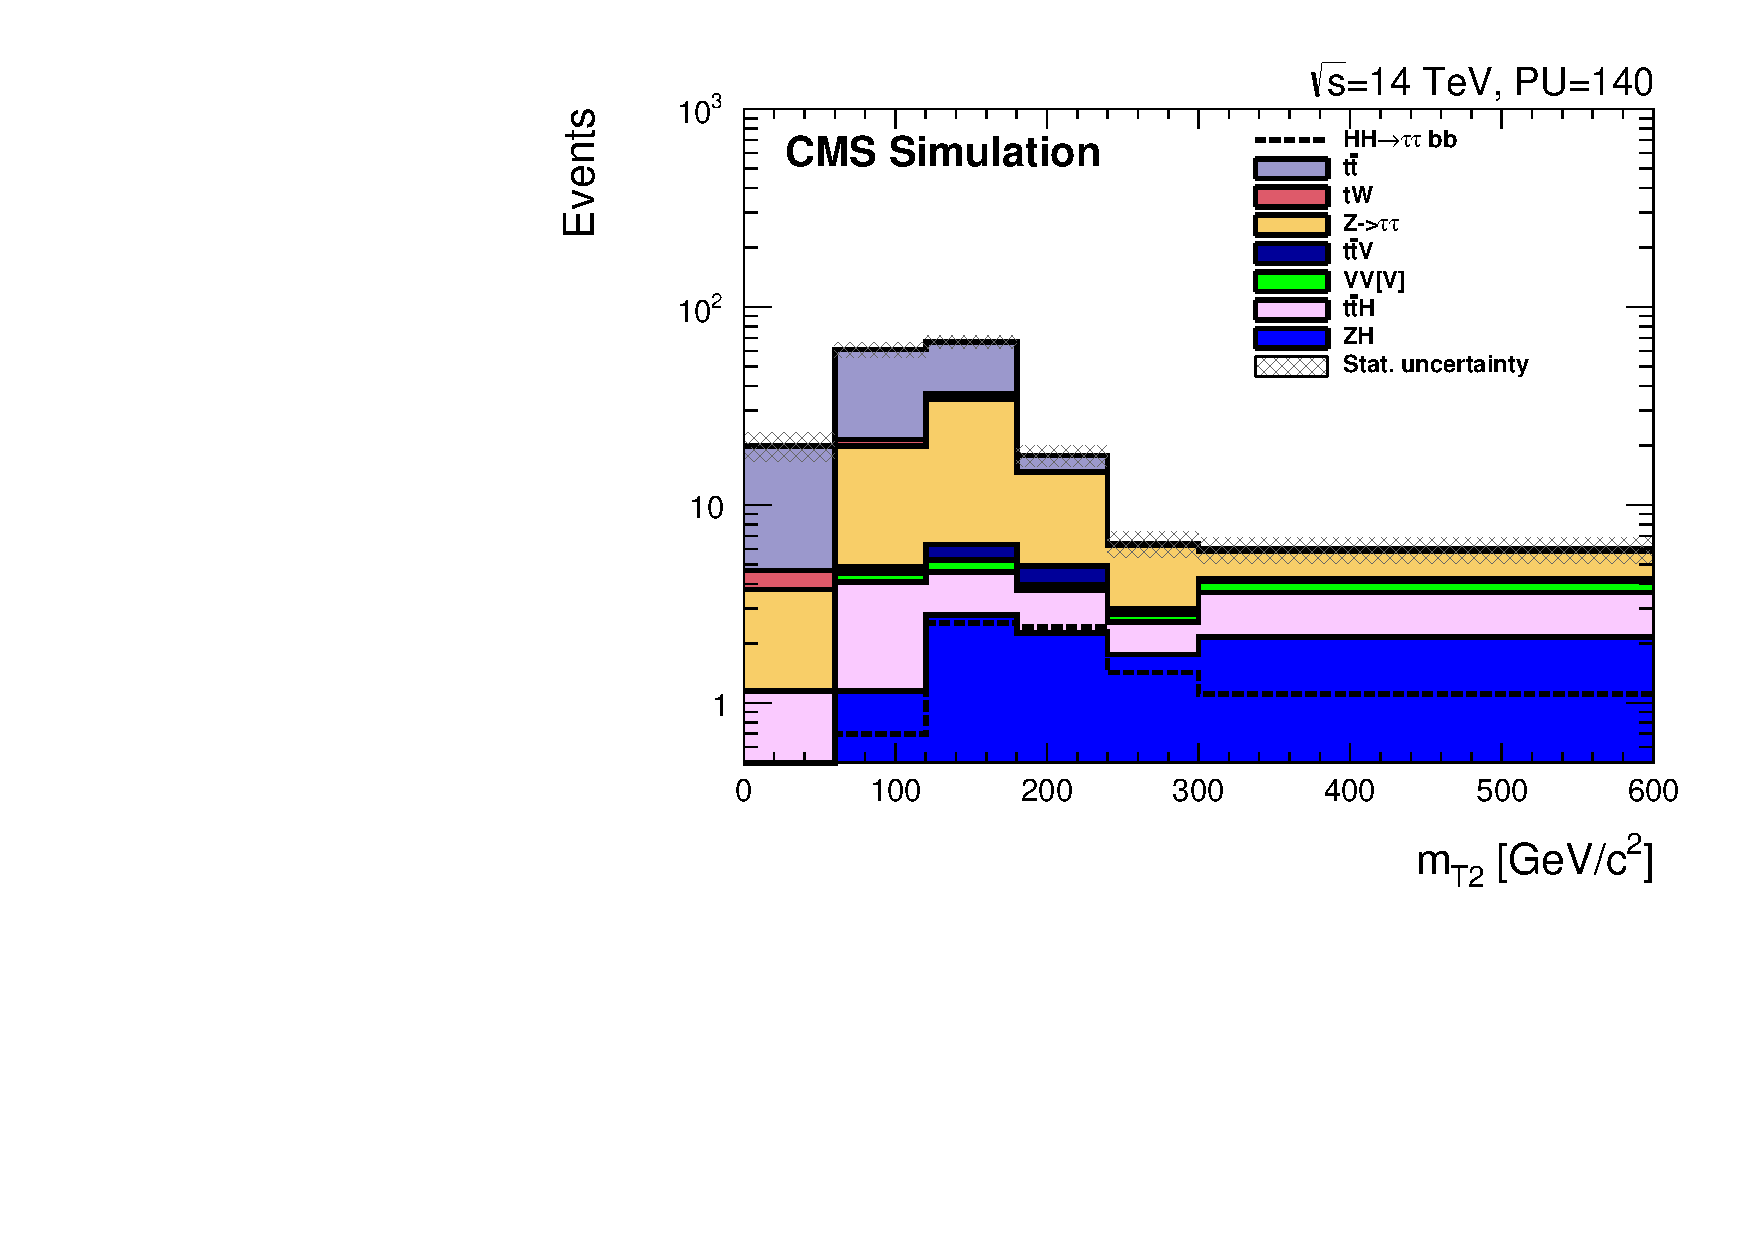
\includegraphics[width=0.49\textwidth]{figures_chapter6/thth_mt2.pdf}   
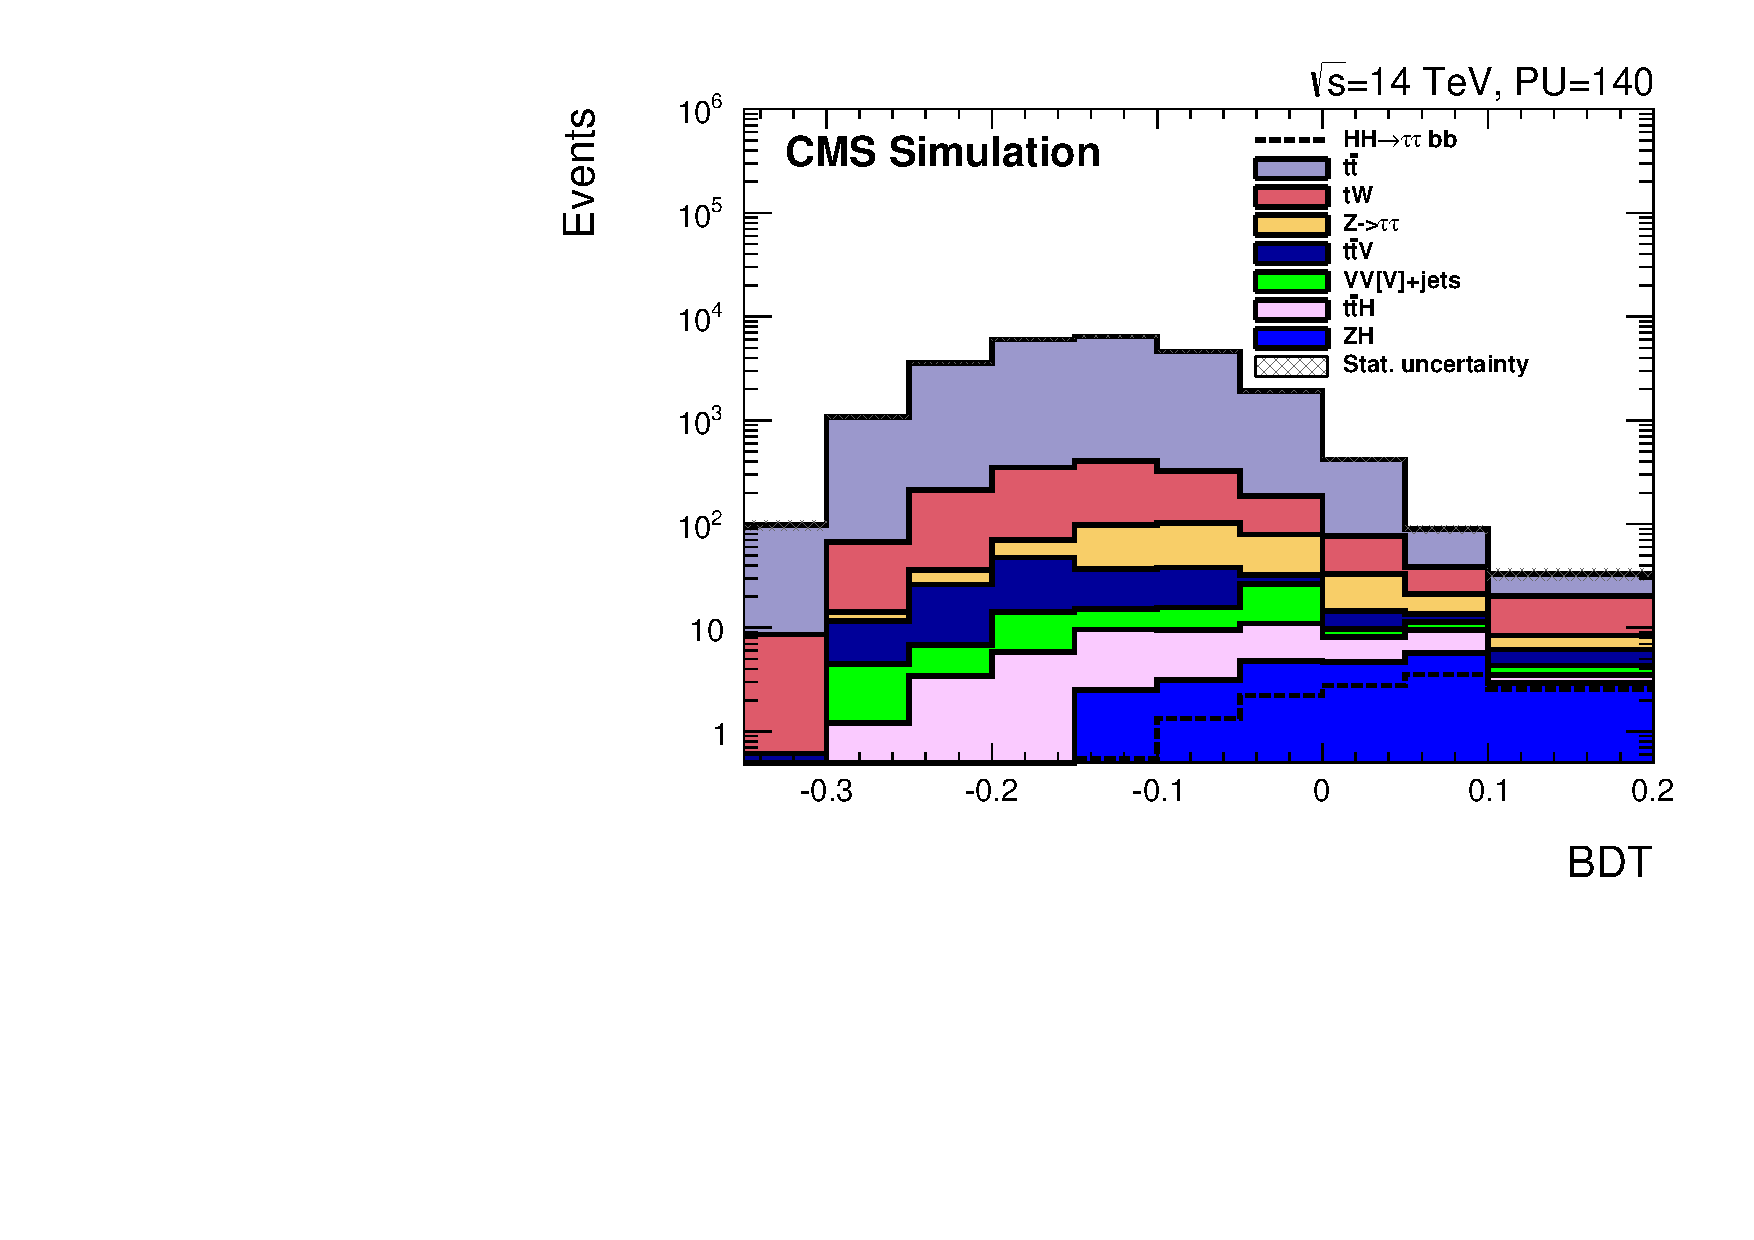
\includegraphics[width=0.49\textwidth]{figures_chapter6/tmth_bdt.pdf}
\caption{$m_{T2}$ (left) and BDT score (right) distributions in  $\tau_{h}\tau_{h}$ and  $\tau_{\mu}\tau_{h}$ channels, respectively. The yields are the expected SM 
contributions.}
\label{fig:bdtout}
\end{center}
\end{figure}

The expected significance for the di-Higgs boson production is $0.5$ and $0.7$ standard deviations, for
$\tau_{\mu}\tau_{h}$ and $\tau_{h}\tau_{h}$ di-tau final states,
respectively. For the combination, $0.9$ standard deviations are expected. The resulting expected
uncertainty in the signal strength is approximately
$105\%$. Theoretical uncertainties in the Higgs boson production are
included in this result. Renormalization and factorization scale
uncertainties in the di-Higgs boson signal production are $20\%$ for NNLO
calculation. The PDF uncertainty is $9\%$. The systematic uncertainty in
the luminosity is taken to be $2.6\%$. Energy scale uncertainties on jets, tau
leptons, and missing energy are also included. A scale uncertainty of $2\%$ is assumed which is comparable to the corresponding uncertainty for Run1 conditions~\cite{CMS-DP-2013-011} in the barrel and endcap regions. The effect of the jet energy scale uncertainty in the sensitivity is about $5\%$.       

\begin{table}[!ht]
\begin{center} 
\begin{tabular}{|c|c|c|c|c|}
\hline
Selection  & $HH$ & $ZH$ & $t\bar{t}H$ & $Z\rightarrow \tau\tau$  \\  \hline
Baseline selection & $23.6\pm0.5$ & $104.7\pm3.5$ & $204.6\pm5.8$ & $479.3\pm7.7$  \\
Mass windows  & $8.3\pm0.3$ & $10.1\pm1.0$ & $9.8\pm1.3$ & $60.3\pm3.3$ \\ 
Signal  & $4.9\pm0.2$ & $6.2\pm0.8$ &  $3.8\pm0.8$ & $14.7\pm1.6$ \\ \hline
\end{tabular}

\vspace{2mm}

\begin{tabular}{|c|c|c|c|c|}
\hline
Selection   & $t\bar{t}$ & $tW$ & $t\bar{t}V$ & $VV(V)$  \\  \hline
Baseline selection & $7662\pm69$ & $734.4\pm19.4$ & $189.4\pm10.0$ & $128.9\pm16.7$  \\
Mass windows  & $88.4\pm7.5$ & $4.8\pm1.6$ & $2.7\pm0.9$ & $2.1\pm0.7$ \\ 
Signal  & $3.2\pm1.4$ & $0.1\pm0.1$ & $1.3\pm0.7$ & $1.0\pm0.5$ \\ \hline
\end{tabular}

\caption{ The expected signal yields for $3000$~$\mathrm{fb}^{-1}$ of integrated luminosity are shown at various stages of the cut-based selection in the $\tau_{h}\tau_{h}$ channel. A loose mass window cut is applied on the $t\bar{t}$ sample at the  generation level. For the signal selection stage we require $m_{T2}$ to be greater than $180$~GeV. The full $m_{T2}$ distribution is used for the signal extraction.}
\label{tab:hhsig}
\end{center}
\end{table}


\begin{table}[!ht]
\begin{center} 
\begin{tabular}{|c|c|c|c|c|}
\hline
Selection  & $HH$ & $ZH$ & $t\bar{t}H$ & $Z\rightarrow \tau\tau$  \\  \hline 
Baseline selection & $39.2\pm0.6$ & $213.7\pm4.7$ & $1175.8\pm12.9$ & $3711.7\pm34.1$  \\
Mass window  & $13.1\pm0.4$ & $24.4\pm1.5$ & $37.7\pm2.3$ & $234.5\pm8.6$  \\ 
Signal  & $6.1\pm0.3$ & $8.6\pm0.9$ & $4.5\pm0.8$ & $9.7\pm1.7$ \\ \hline
\end{tabular}

\vspace{2mm}

\begin{tabular}{|c|c|c|c|c|}
\hline
Selection  & $t\bar{t}$ & $tW$ & $t\bar{t}V$ & $VV(V)$  \\  \hline
Baseline selection & $(3.84\pm0.00)\times10^{5}$ & $(3.72\pm0.00)\times10^{4}$ & $4154\pm39$ & $1418\pm90$ \\
Mass window   & $(2.3\pm0.0)\times10^{4}$ & $1232\pm33$ & $119.4\pm7.4$ & $49.6\pm2.3$   \\ 
Signal   & $63.5\pm7.3$ & $29.2\pm4.8$ & $3.9\pm1.3$  & $2.7\pm0.7$ \\ \hline
\end{tabular}

\caption{ The expected signal yields for $3000$~$\mathrm{fb}^{-1}$ of integrated luminosity are shown at various stages of the cut-based selection in the $\tau_{\mu}\tau_{h}$ channel. A loose mass window cut is applied on the $t\bar{t}$ sample at the generation level. For the signal selection stage we require the BDT variable to be greater than $0.05$. The full BDT distribution is used for the signal extraction.}
\label{tab:mhsig}
\end{center}
\end{table}

\subsection{Trigger performance}
The performance of the trigger system is crucial to achieve the result
described above, in particular the capability to trigger on charged
particles at Level-1. For the $\tau_{h}\tau_{h}$ final state, the
di-tau trigger has an offline threshold of $56$~GeV on both tau legs,
and the single tau trigger threshold is $88$~GeV for the Level-1 sample menu
described in this document. These thresholds are significantly higher
without the track trigger, $95$~GeV on both tau legs for the di-tau
trigger and $138$~GeV for the single tau trigger. Considering these less
performant thresholds, the signal and background yields are reduced by about a factor of
two. For the $\tau_{\mu}\tau_{h}$ final state the situation is similar. The single-muon trigger
threshold is $18$~GeV with the track trigger and $50$~GeV without the track
trigger. The thresholds for the muon-tau trigger legs are significantly
higher as well. Again, the signal and background yields are reduced by a factor of two
by requiring $50$~GeV cut on the $p_T$ of the muon and hadronic tau.
Thus, in both final states the effect of the trigger performance on the sensitivity of this analysis is significant. The overall sensitivity is
reduced by 40\%, the equivalent of  using only half of 3000~fb$^{-1}$.

\section{Combination of $bb\gamma\gamma$ and $bb\tau\tau$ results}
A combination of the  $bb\gamma\gamma$ and $bb\tau\tau$ results is performed by performing a simultaneous fit to the generated pseudo-data. A test statistic based on the profile likelihood ratio is used. Systematic uncertainties are incorporated through nuisance parameters and are treated according to frequentist paradigm. A detailed description of the methodology is given in Refs.~\cite{CMS-NOTE-2011-005,Chatrchyan201226}. The expected uncertainty in the signal yield is approximately $54\%$. The expected significance for di-Higgs boson production is $1.9$ standard deviations.  

\section{Summary}
\label{sec:conclusion}
Studies  of the Higgs boson pair production and decays into $bb\gamma\gamma$ and $bb\tau\tau$ final states are presented. The studies are performed assuming the operational conditions of the HL-LHC, with an integrated luminosity of 3000~$\mathrm{fb}^{-1}$, and the upgraded CMS experiment. Combining the studies of $bb\gamma\gamma$ and $bb\tau\tau$ final states, the expected significance for Higgs boson pair production is 1.9 standard deviation. The resulting expected uncertainty in the signal yield is $54\%$. We emphasized the benefits of the CMS \phasetwo upgrades to meet the challenges presented by high luminosity environment. Further improvements of the sensitivity are possible by using more sophisticated reconstruction and analysis techniques. Additional di-Higgs boson production and decay modes remain unexplored. Among these the bbbb final state promises the largest potential for improvement.

%\section{Higgs CP in e+e- colliders}
